\chapter{Design and model}
\label{designModel}

In this chapter we will focus in the description of the mechanical model of the UAV and the sensor system and, from these, a mathematical model will be derived, necessary for build and simulate a control law, and to perform system identification.

\section{Mechanical design}
\label{mechanicalDesign}

The overall objective of the Prometheus project is navigation and mapping, for these we mean obtain a 3D reconstruction of an unknown indoor physical environment, using a 360 degrees \textit{Lidar} laser scanner, which, coupled to a quadrotor type UAV, will explore in a autonomus way. Lidar is a surveying technology that measures distance by illuminating a target with a laser light. Lidar is an acronym of Light Detection And Ranging, (sometimes Light Imaging, Detection, And Ranging). 

\begin{SCfigure}[\sidecaptionrelwidth][h]
	\includegraphics[scale=0.21]{images/lidar_laser.jpg}
	\caption{Lidar laser scanner, it is able to perform a 360 degrees mapping.}
	\label{fig:lidar}
\end{SCfigure}

\noindent Lidar is popularly used as a technology to make high-resolution maps, with applications in geodesy, geomatics, archaeology, geography, geology, geomorphology, seismology, forestry, atmospheric physics and so on. What is known as Lidar is sometimes simply referred to as laser scanning or 3D scanning, with terrestrial, airborne and mobile applications \footnote{\url{https://en.wikipedia.org/wiki/Lidar}}. The specific Lidar laser scanner used in this project is depict in figure \ref{fig:lidar}, where is possible to see the rotating structure moved by a motor attached in the bottom of the frame. However, this sensor is only able to perform 2D mapping and, attached to a drone, make it practically impossible to perform a complete 3D mapping. To solve this problem, several approaches could be adopted, such as use a more complicated and more expensive sensor, that can maps direclty in 3D, or just by simply use more than one Lidar. However, the solution adopted in this project is again inspired from the movie Prometheus, where the sensor is also rotating around the UAV. In such a way, the Lidar has three degrees of freedom in the movement and a 3D mapping can be performed. This solution comports, of course,the usage of only one laser scanner, but require a rotating structure that can move the sensor.

\textcolor{red}{Add renders here.}

\noindent In figure [\textcolor{red}{renders}] is possible to see clearly the platform, made of two lightweight rings, and the cart that provides the circular movement of the sensor. An important choice was also the selection of the UAV, that has to guarantee to flight also with the weight of the mechanical structure, sensor and all the electronics needed to fly and control the movement of the cart.

\section{Mathematical model}
\label{mathematicalModel}

Is pretty much clear from the previous section that this UAV is different from almost every other vehicle that is possible to buy, this of course require a complete and detailed study to characterize the mathematical model. For characterize the model, is before necessary to provide some definitions, that are also valid for standar commercial quadrotors.

\begin{figure}[h]
	\centering
	\tdplotsetmaincoords{50}{-60} % 50 -60
		
	\def \semiaxis  {0.8}					% from center to propeller (diag)
	\def \centers {\semiaxis}		        % x and y of centers
	\def \body {\semiaxis / 5}				% half diagonal of body
	\def \height {0.05}						% half height of body
	\def \propeller {0.3}					% radius of propeller
	\def \innerpropeller {0.05}				% radius inner circle propeller
	\def \heightpropeller {0.05}			% height propeller plane
		
	\begin{tikzpicture}[scale=4,tdplot_main_coords]
		
		% axis
		\draw[line width=3pt] (-\centers, 0, 0) -- (\centers, 0, 0);	
		\draw[line width=3pt] (0, \centers, 0) -- (0, -\centers, 0);

		% propellers
		\tdplotdrawarc[thick, fill=gray] {(0, \centers, \heightpropeller)}{\propeller}{0}{360}{}{}
		\tdplotdrawarc[thick, fill=gray] {(\centers, 0, \heightpropeller)}{\propeller}{0}{360}{}{}
		\tdplotdrawarc[thick, fill=gray] {(0, -\centers, \heightpropeller)}{\propeller}{0}{360}{}{}
		\tdplotdrawarc[thick, fill=gray] {(-\centers, 0, \heightpropeller)}{\propeller}{0}{360}{}{}

		% center propellers
		\tdplotdrawarc[fill] {(0, \centers, \heightpropeller)}{\innerpropeller}{0}{360}{}{}
		\tdplotdrawarc[fill] {(\centers, 0, \heightpropeller)}{\innerpropeller}{0}{360}{}{}
		\tdplotdrawarc[fill] {(0, -\centers, \heightpropeller)}{\innerpropeller}{0}{360}{}{}
		\tdplotdrawarc[fill] {(-\centers, 0, \heightpropeller)}{\innerpropeller}{0}{360}{}{}

		% body
		\fill (\body,\body,\height) -- (\body,-\body,\height) -- (-\body,-\body,\height) -- (-\body,\body,\height) -- cycle;
		\fill (\body,\body,-\height) -- (\body,-\body,-\height) -- (-\body,-\body,-\height) -- (-\body,\body,-\height) -- cycle; % down
		\fill (-\body,-\body,-\height) -- (-\body,-\body,\height) -- (-\body,\body,\height) -- (-\body,\body,-\height) -- cycle; % back
		\fill (\body,\body,-\height) -- (\body,\body,\height) -- (\body,-\body,\height) -- (\body,-\body,-\height) -- cycle; % front
		\fill (\body,-\body,-\height) -- (\body,-\body,\height) -- (-\body,-\body,\height) -- (-\body,-\body,-\height) -- cycle; % left
		\fill (\body,\body,-\height) -- (\body,\body,\height) -- (-\body,\body,\height) -- (-\body,\body,-\height) -- cycle; % right
		
		% Coordinate frame
		\coordinate (O) at (0,0,0) node[red, anchor = north]{$O_B$};
		\draw[ultra thick,->,red] (0,0,0) -- (0,-1.1,0) node[anchor=north west]{$x_B$};
		\draw[ultra thick,->,red] (0,0,0) -- (1.1,0,0) node[anchor=south west]{$y_B$};
		\draw[ultra thick,->,red] (0,0,0) -- (0,0,1.1) node[anchor=south]{$z_B$};

		% Rotors arrows
		\draw [->, ultra thick] (\centers+0.2, 0, \heightpropeller) arc (0:300:0.2);
		\draw [->, ultra thick] (-\centers+0.2, 0, \heightpropeller) arc (0:300:0.2);
		\draw [<-, ultra thick] (0.2, \centers, \heightpropeller) arc (0:300:0.2);
		\draw [<-, ultra thick] (0.2, -\centers, \heightpropeller) arc (0:300:0.2);				
	\end{tikzpicture}
	\caption{Sketch of a standard quadrotor with its body frame attach.}
	\label{fig:quadrtotor}
\end{figure}

\noindent A quadrotor helicopter is made of a central frame and four propellers that are attach to the frame with respectively four arms. Moreover, the propellers' rotation direction must be opposite in pairs, like illustrated in figure \ref{fig:quadrtotor}. \newline
\noindent Furthermore, is necessary to define two frames, the world fixed frame and the body frame attached to the vehicle.

\begin{figure}[h]
	\centering
	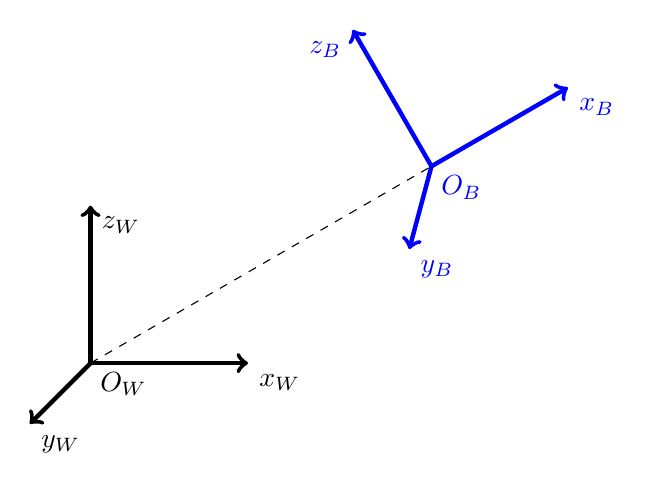
\begin{tikzpicture}[]

		\def \length {2}
		\def \xbody {5}
		\def \ybody {0}

		% World frame
		\draw[rotate=30] (0, 0, 0) -- (0, 0, 0) node[anchor=north west]{$O_W$};
		\draw[->, ultra thick] (0, 0, 0) -- (\length, 0, 0) node[anchor=north west]{$x_W$};
		\draw[->, ultra thick] (0, 0, 0) -- (0, \length, 0) node[anchor=north west]{$z_W$};
		\draw[->, ultra thick] (0, 0, 0) -- (0, 0, \length) node[anchor=north west]{$y_W$};

		% Body frame
		\draw[rotate=30] (\xbody, \ybody, 0) -- (\xbody, \ybody, 0) node[anchor=north west, blue]{$O_B$};
		\draw[->, ultra thick, blue, rotate=30] (\xbody, \ybody, 0) -- (\xbody+\length, \ybody, 0) node[anchor=north west]{$x_B$};
		\draw[->, ultra thick, blue, rotate=30] (\xbody, \ybody, 0) -- (\xbody, \ybody+\length, 0) node[anchor=north east]{$z_B$};
		\draw[->, ultra thick, blue, rotate=30] (\xbody, \ybody, 0) -- (\xbody, \ybody, \length) node[anchor=north west]{$y_B$};

		\draw[-, dashed, rotate=30] (0, 0, 0) -- (\xbody, \ybody, 0);

	\end{tikzpicture}
	\caption{Illustration of the world and body frames. \textcolor{red}{Maybe change the inclination}
}
	\label{fig:frames}
\end{figure}

\noindent In figure \ref{fig:frames} is possible to see the two frames, the world frame, in black, is fixed to a point and it can't be moved, the body frame, in blue, instead is attached to the quadrotor and can move with six degrees of freedom, that are position and orientation. In this, we are interesting in knowing the traslation and rotation of the body frame in respect to the world frame. For rappresent the traslation, a three dimension vector $\mathbf{x}$ is enough, that actually indicate the position of the quadrotor in the space. Instead, for the rotation, we used quaternions \cite{quaternion}, that will be introduced in the following section.

	
\subsection{Quaternion math}
\label{quaternion}

A quaternion is a hyper complex number of rank 4, which can be represented as follow

\begin{equation}
	\mathbf{q} = 
	\begin{bmatrix}
		q_0 & q_1 & q_2 & q_3
	\end{bmatrix}^T
	\label{eq:quatDef}
\end{equation}

\noindent The quaternion units from $q_1$ to $q_3$ are called the vector part of the quaternion, while $q_0$ is the scalar part \cite{EmilQuaternion}. Multiplication of two quaternions $\mathbf{p}$ and $\mathbf{q}$, is being performed by the Kronecker product, denoted as $\otimes$. If $\mathbf{p}$ represents one rotation and $\mathbf{q}$ represents another rotation, then $\mathbf{p} \otimes \mathbf{q}$ represents the combined rotation.

\begin{align}
	\mathbf{p} \otimes \mathbf{q} &=
	\begin{bmatrix}
		p_0q_0 - p_1q_1 - p_2q_2 - p_3q_3 \\
		p_0q_1 + p_1q_0 + p_2q_3 - p_3q_2 \\
		p_0q_2 - p_1q_3 + p_2q_0 + p_3q_1 \\
		p_0q_3 + p_1q_2 - p_2q_1 + p_3q_0
	\end{bmatrix} \\
	&= Q(\mathbf{p})\mathbf{q} =
	\begin{bmatrix}
		p_0 & -p_1 & -p_2 & -p_3 \\
		p_1 & p_0  & -p_3 & p_2 \\
		p_2 & p_3  & p_0  & -p_1 \\
		p_3 & -p2  & p_1  & p_0
	\end{bmatrix}
	\begin{bmatrix}
		q_0 \\
		q_1 \\
		q_2 \\
		q_3
	\end{bmatrix} \\
	&= \bar{Q}(\mathbf{q})\mathbf{p} = 
	\begin{bmatrix}
		q_0 & -q_1 & -q_2 & -q_3 \\
		q_1 & q_0  & q_3  & -q_2 \\
		q_2 & -q_3 & q_0  & q_1 \\
		q_3 & q_2  & -q_1 & q_0  
	\end{bmatrix}
	\begin{bmatrix}
		p_0 \\
		p_1 \\
		p_2 \\
		p_3
	\end{bmatrix}
	\label{eq:quatKronecker}
\end{align}

\noindent The norm of a quaternion is defined as

\begin{equation}
	||\mathbf{q}|| = \sqrt{q_0^2 + q_1^2 + q_2^2 + q_3^2} 
	\label{eq:quatNorm}
\end{equation}

\noindent If the norm of the quaternion is equal to $1$, then the quaternion is called unit quaternion. The complex conjugate of a quaternion has the same definition as normal complex numbers.

\begin{equation}
	\mathbf{q}^* = 
	\begin{bmatrix}
		q_0 & -q_1 & -q_2 & -q_3
	\end{bmatrix}^T
	\label{eq:quatConj}
\end{equation}

\noindent The inverse of a quaternion is defined as a normal inverse of a complex number.

\begin{equation}
	\mathbf{q}^{-1} = \frac{\mathbf{q}^*}{||\mathbf{q}||^2}
	\label{eq:quatInverse}
\end{equation}

\noindent The time derivative of the unit quaternion is the vector of quaternion rates \cite{quaternion2}. It requires some algebraic manipulation but is important to notice that the quaternion rates, $\dot{\mathbf{q}}$, are related to the angular velocity $\boldsymbol{\omega} = \begin{bmatrix} \omega_x & \omega_y & \omega_z \end{bmatrix}^T$. It can be represented in two ways:

\begin{itemize}
		
	\item as in equation \eqref{eq:quatDerivative1} in case that the angular velocity is in the world frame
	\begin{equation}
		\dot{\mathbf{q}}_{\boldsymbol{w}}(\mathbf{q}, \boldsymbol{w}) = \frac{1}{2}\mathbf{q}\otimes
		\begin{bmatrix}
			0 \\
			\boldsymbol{\omega}
		\end{bmatrix}
		= \frac{1}{2}Q(\mathbf{q})
		\begin{bmatrix}
			0 \\
			\boldsymbol{\omega}
		\end{bmatrix}
		\label{eq:quatDerivative1}
	\end{equation}

	\item as in equation \eqref{eq:quatDerivative2} if the angular velocity vector is in the body frame of reference.

	\begin{equation}
		\dot{\mathbf{q}}_{\boldsymbol{w}'}(\mathbf{q}, \boldsymbol{w}') = \frac{1}{2}
		\begin{bmatrix}
			0 \\
			\boldsymbol{\omega}'
		\end{bmatrix}
		\otimes \mathbf{q} = \frac{1}{2}\bar{Q}(\mathbf{q})
		\begin{bmatrix}
			0 \\
			\boldsymbol{\omega}'
		\end{bmatrix}
		\label{eq:quatDerivative2}
	\end{equation}
\end{itemize}

\noindent A unit quaternion can be used also as a rotation operator, however the transformation requires both the quaternion and its conjugate, as show in equation \eqref{eq:quatRotateVector}. This rotates the vector $\mathbf{v}$ from the world frame to the body frame represented by $\mathbf{q}$.

\begin{equation}
	\boldsymbol{\omega} = \mathbf{q} \otimes 
	\begin{bmatrix}
		0 \\
		\mathbf{v}
	\end{bmatrix}
	\otimes \mathbf{q}^*
	\label{eq:quatRotateVector}
\end{equation}

\noindent Unit quaternion can be use also to represents rotation matrixes. Consider a vector $\mathbf{v}$ in the world frame. If $\mathbf{v}'$ is the same vector in the body coordinates, the the following relations hold

\begin{align}
	\begin{bmatrix}
		0 \\
		\mathbf{v}'
	\end{bmatrix}
	&= \mathbf{q} \cdot
	\begin{bmatrix}
		0 \\
		\mathbf{v}
	\end{bmatrix}
	\cdot \mathbf{q}^* \\
	&= \bar{Q}(\mathbf{q})^T Q(\mathbf{q})
	\begin{bmatrix}
		0 \\
		\mathbf{v}
	\end{bmatrix} \\
	&=
	\begin{bmatrix}
		1          & \mathbf{0}^T \\
		\mathbf{0} & R_{\mathbf{q}}(\mathbf{q})
	\end{bmatrix}
	\begin{bmatrix}
		0 \\
		\mathbf{v}
	\end{bmatrix}
	\label{eq:quatRotationMatrix1}
\end{align}

\noindent where

\begin{equation}
	R_{\mathbf{q}}(\mathbf{q}) =
	\begin{bmatrix}
		q_0^2+q_1^2-q_2^2-q_3^2 & 2q_1q_2+2q_0q_3         & 2q_1q_3-2q_0q_2 \\
		2q_1q_2-2q_0q_3         & q_0^2-q_1^2+q_2^2-q_3^2 & 2q_2q_3+2q_0q_1 \\
		2q_1q_3+2q_0q_2         & 2q_2q_3-2q_0q_1         & q_0^2-q_1^2-q_2^2+q_3^2
	\end{bmatrix}
	\label{eq:quatRotationMatrix2}
\end{equation}

\noindent That is,

\begin{align}
	\mathbf{v}' &= R_{\mathbf{q}}(\mathbf{q})\mathbf{v} \\
	\mathbf{v} &= R_{\mathbf{q}}(\mathbf{q})^T\mathbf{v}'
	\label{eq:quatRotationMatrix3}
\end{align}

\noindent Just as with rotation matrices, sequences of rotations are represented by products of quaternions. That is, for unit quaternions $\mathbf{q}$ and $\mathbf{p}$, it holds that

\begin{equation}
	R_{\mathbf{q}}(\mathbf{q} \cdot \mathbf{p}) = R_{\mathbf{q}}(\mathbf{q})R_{\mathbf{q}}(\mathbf{p})
	\label{eq:quatRotationMatrix4}
\end{equation}

\noindent Finally, for representing quaternion rotations in a more intuitive manner, the conversion from Euler angles (roll $\phi$, pith $\theta$ and yaw $\psi$) to quaternion and viceversa can be performed by utilizing the following two equations respectively.

\begin{gather}
	q = 
	\begin{bmatrix}
		\cos{(\phi/2)}\cos{(\theta/2)}\cos{(\psi/2)} + \sin{(\phi/2)}\sin{(\theta/2)}\sin{(\psi/2)} \\
		\sin{(\phi/2)}\cos{(\theta/2)}\cos{(\psi/2)} - \cos{(\phi/2)}\sin{(\theta/2)}\sin{(\psi/2)} \\
		\cos{(\phi/2)}\sin{(\theta/2)}\cos{(\psi/2)} + \sin{(\phi/2)}\cos{(\theta/2)}\sin{(\psi/2)} \\
		\cos{(\phi/2)}\cos{(\theta/2)}\sin{(\psi/2)} - \sin{(\phi/2)}\sin{(\theta/2)}\cos{(\psi/2)} 
	\end{bmatrix} \\
	\begin{bmatrix}
		\phi \\
		\theta \\
		\psi
	\end{bmatrix}
	=
	\begin{bmatrix}
		\atan2(2(q_0q_1+q_2q_3), q_0^2-q_1^2-q_2^2+q_3^2) \\
		\asin(2(q_0q_2-q_3q_1)) \\
		\atan2(2(q_0q_3+q_1q_2), q_0^2+q_1^2-q_2^2-q_3^2)
	\end{bmatrix}
	\label{eq:quatEuler}
\end{gather}

\phantom{x} % necessary to place the next figure

\subsection{Quadrotor modelling}
\label{quadModel}

We consider first a standard quadrotor, without a rotating platform, like in figure \ref{fig:quadrtotorVectors}. 

\begin{figure}[!h]
	\centering
	\tdplotsetmaincoords{60}{-135} % 60 -135
		
	\def \semiaxis  {0.8}			    	% from center to propeller (diag)
	\def \centers {\semiaxis}		        % x and y of centers
	\def \body {\semiaxis / 5}				% half diagonal of body
	\def \height {0.05}						% half height of body
	\def \propeller {0.3}					% radius of propeller
	\def \innerpropeller {0.05}				% radius inner circle propeller
	\def \heightpropeller {0.05}			% height propeller plane
		
	\begin{tikzpicture}[scale=4,tdplot_main_coords]
		
		% axis
		\draw[line width=3pt] (-\centers, 0, 0) -- (\centers, 0, 0);	
		\draw[line width=3pt] (0, \centers, 0) -- (0, -\centers, 0);

		% propellers
		\tdplotdrawarc[thick, fill=gray] {(0, \centers, \heightpropeller)}{\propeller}{0}{360}{}{}
		\tdplotdrawarc[thick, fill=gray] {(\centers, 0, \heightpropeller)}{\propeller}{0}{360}{}{}
		\tdplotdrawarc[thick, fill=gray] {(0, -\centers, \heightpropeller)}{\propeller}{0}{360}{}{}
		\tdplotdrawarc[thick, fill=gray] {(-\centers, 0, \heightpropeller)}{\propeller}{0}{360}{}{}

		% center propellers
		\tdplotdrawarc[fill] {(0, \centers, \heightpropeller)}{\innerpropeller}{0}{360}{}{}
		\tdplotdrawarc[fill] {(\centers, 0, \heightpropeller)}{\innerpropeller}{0}{360}{}{}
		\tdplotdrawarc[fill] {(0, -\centers, \heightpropeller)}{\innerpropeller}{0}{360}{}{}
		\tdplotdrawarc[fill] {(-\centers, 0, \heightpropeller)}{\innerpropeller}{0}{360}{}{}

		% body
		\fill (\body,\body,\height) -- (\body,-\body,\height) -- (-\body,-\body,\height) -- (-\body,\body,\height) -- cycle;
		\fill (\body,\body,-\height) -- (\body,-\body,-\height) -- (-\body,-\body,-\height) -- (-\body,\body,-\height) -- cycle; % down
		\fill (-\body,-\body,-\height) -- (-\body,-\body,\height) -- (-\body,\body,\height) -- (-\body,\body,-\height) -- cycle; % back
		\fill (\body,\body,-\height) -- (\body,\body,\height) -- (\body,-\body,\height) -- (\body,-\body,-\height) -- cycle; % front
		\fill (\body,-\body,-\height) -- (\body,-\body,\height) -- (-\body,-\body,\height) -- (-\body,-\body,-\height) -- cycle; % left
		\fill (\body,\body,-\height) -- (\body,\body,\height) -- (-\body,\body,\height) -- (-\body,\body,-\height) -- cycle; % right
		
		% Coordinate frame
		\coordinate (O) at (0,0,0) node[red, anchor=east]{$O_B$};
		\draw[ultra thick,->,red] (0,0,0) -- (0,-1.6,0) node[anchor=south west]{$x_B$};
		\draw[ultra thick,->,red] (0,0,0) -- (1.6,0,0) node[anchor=east]{$y_B$};
		\draw[ultra thick,->,red] (0,0,0) -- (0,0,1.4) node[anchor=south]{$z_B$};

		% Rotors arrows
		\draw [->, ultra thick] (\centers+0.2, 0, \heightpropeller) arc (0:300:0.2) node[anchor=south west]{$\Omega_4$};
		\draw [->, ultra thick] (-\centers+0.2, 0, \heightpropeller) arc (0:300:0.2) node[anchor=south west]{$\Omega_2$};
		\draw [<-, ultra thick] (0.2, \centers, \heightpropeller) arc (0:300:0.2) node[anchor=south west]{$\Omega_3$};
		\draw [<-, ultra thick] (0.2, -\centers, \heightpropeller) arc (0:300:0.2) node[anchor=south west]{$\Omega_1$};

		% Force arrows
		\draw[ultra thick,->,blue] (0, \centers, \heightpropeller) -- (0, \centers, \heightpropeller+0.4) node[anchor=east]{$F_3$};
		\draw[ultra thick,->,blue] (\centers, 0, \heightpropeller) -- (\centers, 0, \heightpropeller+0.4) node[anchor=east]{$F_4$};
		\draw[ultra thick,->,blue] (0, -\centers, \heightpropeller) -- (0, -\centers, \heightpropeller+0.4) node[anchor=east]{$F_1$};
		\draw[ultra thick,->,blue] (-\centers, 0, \heightpropeller) -- (-\centers, 0, \heightpropeller+0.4) node[anchor=east]{$F_2$};

		% Torque arrows
        \draw[->, ultra thick, canvas is zy plane at x=\centers+0.6, orange] (0.15, 0, 0) arc (0:360:0.15) node[anchor=south east]{$\tau_y$};
        \draw[->, ultra thick, canvas is zx plane at y=-\centers-0.6, orange] (0.15, 0, 0) arc (0:360:0.15) node[anchor=south east]{$\tau_x$};
        \draw[->, ultra thick, orange] (0.15, 0, 0.6) arc (0:360:0.15) node[anchor=south east]{$\tau_z$};

	\end{tikzpicture}
	\caption{Sketch of a standard quadrotor.}
	\label{fig:quadrtotorVectors}
\end{figure}

\noindent In fiure \ref{fig:quadrtotorVectors} are also impres the force vectors $F_i$ generate from each motor-propeller, the torques vectors $\tau_x$, $\tau_y$ and $\tau_z$ about the three axis and the propeller's speed $\Omega_i$. Now, for modeling the rigid body of a multirotor, the standard Newton-Euler kinematics equations can be utilized \cite{Bresciani}.

\begin{equation}
	\begin{bmatrix}
		\mathbf{F} \\
		\boldsymbol{\tau}
	\end{bmatrix}
	=
	\begin{bmatrix}
		m \cdot I_{3\times 3} & \mathbf{0} \\
		\mathbf{0}^T & I_{cm}
	\end{bmatrix}
	\begin{bmatrix}
		\mathbf{\ddot{x}_B} \\
		\boldsymbol{\dot{\omega}_B}
	\end{bmatrix}
	+
	\begin{bmatrix}
		\mathbf{0} \\
		\boldsymbol{\omega_B} \times I_{cm} \cdot \boldsymbol{\omega_B}
	\end{bmatrix}
	\label{eq:NewtonEuler}
\end{equation}

\noindent Where $\mathbf{F} = \begin{bmatrix} F_x & F_y & F_z \end{bmatrix}^T$ is the vector of the total force, $\boldsymbol{\tau} = \begin{bmatrix} \tau_x & \tau_y & \tau_z \end{bmatrix}^T$ is the total torque, $m$ is the mass of the quadrtotor, $I_{cm}$ is the matrix of inertia related to the center of mass, $\mathbf{\ddot{x}_B}$ is the acceleration of the quadrotor center of mass related to the body frame and $\boldsymbol{\omega_B} = \begin{bmatrix} \omega_x & \omega_y & \omega_z \end{bmatrix}^T$ is the rotational rates in the body frame.

\noindent Before deriving the torque relationship, the motors' models from the input signal to the thrust force are needed. In specific, the four input signals are the speed of the propellers $u_i$, map between $0$ (no throttle) and $1$ (full throttle). Then, the thrust for each propeller can be simply derive as follow

\begin{equation}
	F_i(t) = A_{F,i} \Omega_i^2 = A_{F,i}\Omega_{max, i}^2 u_i(t)^2
	\label{eq:motorThrust}
\end{equation}

\noindent where $A_{F,i} \in \rm I\!R_+$ are the thrust constants of the motor-propeller combination, $\Omega_{max, i} \in \rm I\!R_+$ are the maximum rotational speed of the motors and $u_i(t)$ are the motors' signals. What is missing in equation \eqref{eq:motorThrust} is the model of the DC motors and in particular, a map between the input signal $u_i(t)$ and the control signal $u_{in,i}(t)$. To keep the model simple but still accurate \footnote{\url{http://pi19404.github.io/pyVision/2015/04/10/25/}}, the motor has been modeled like a delay, like in equation \eqref{eq:motorDelay}.

\begin{equation}
	u_i(t) \approx \frac{1}{\tau_i s+1}u_{in.i}(t)
	\label{eq:motorDelay}
\end{equation}

\noindent This approach is very common \cite{motor}, since all the parameters of a motor are not provide from datasheet, especially from cheap motors that is possible to find quite often in a commercial quadrotor. Furthermore, to represent the direction of the thrust from a motor it should be considered that 

\begin{align}
	\mathbf{F}_i(t) &= A_{F,i} \Omega_{max,i}^2u_i(t)\mathbf{n}_i \label{eq:propellerDirection1} \\
	\mathbf{n}_i &= R_i \cdot 
	\begin{bmatrix} 
		0 & 0 & 1 
	\end{bmatrix}^T 
	\label{eq:propellerDirection2}
\end{align} 

\noindent Where, in this case, $\mathbf{F}_i(t)$ is the force vector for each propeller and $R_i$ is the rotational matrix encoding the direction of the thrust and torque vector. Then the torque rappresentation is given by

\begin{equation}
	\boldsymbol{\tau}_i(t) = -\sgn(\Omega_i)B_{F,i}\Omega_{max,i}^2u_i(t)^2\mathbf{n}_i
	\label{eq:motorTorque}
\end{equation}

\noindent where $B_{F,i} \in \rm I\!R_+$ is the torque constant.

\noindent Now, by defining the vector $\mathbf{l}_i = \begin{bmatrix} l_{x,i} & l_{y,i} & l_{z,i} \end{bmatrix}^T$ the distance between the center of mass and the position where the propeller $i$ is attached, combining equations \eqref{eq:propellerDirection1}, \eqref{eq:propellerDirection2} and \eqref{eq:motorTorque} is possible to obtain equation \eqref{eq:forceTorque} as in the work \cite{modelIdentification}.

\begin{equation}
	\begin{bmatrix}
		\mathbf{F}_{total} \\
		\boldsymbol{\tau}_{total}
	\end{bmatrix}
	=
	\begin{bmatrix}
		\sum\limits_{i=1}^{4} \mathbf{F}_i(u_i^2) \\
		\sum\limits_{i=1}^{4} \mathbf{l}_i \times \mathbf{F}_i(u_i^2) + \boldsymbol{\tau}_i(u_i^2)
	\end{bmatrix}
	\label{eq:forceTorque}
\end{equation}

\noindent This combined with the Newton-Euler kinematics of equation \eqref{eq:NewtonEuler} gives the final model, from control signal to acceleration and angular acceleration, as depicted in equations \eqref{eq:finalModel1} and \eqref{eq:finalModel2}.

\begin{equation}
	\begin{split}
		\begin{bmatrix}
			\ddot{\mathbf{x}}_B \\
			\dot{\boldsymbol{\omega}}_B
		\end{bmatrix}
		&=
		\begin{bmatrix}
			\dots & \frac{A_{F,i}\Omega_{max,i}^2\mathbf{n}_i}{m} & \dots \\
			\dots & I_{cm}^{-1}\Big[ (\mathbf{l}_i+\boldsymbol{\Delta l})\times A_{F,i}\Omega^2_{max,i}\mathbf{n}_i-\sgn(\Omega_i)B_{F,i}\Omega_{max,i}^2\mathbf{n}_i\Big] & \dots
		\end{bmatrix}
		\begin{bmatrix}
			\vdots \\
			u_i^2 \\
			\vdots
		\end{bmatrix}
		+ \\
		&+
		\begin{bmatrix}
			\mathbf{0} \\
			I_{cm}^{-1}\bigl(\boldsymbol{\omega}_B \times I_{cm} \boldsymbol{\omega}_B \bigl)
		\end{bmatrix} \\
	\end{split}
	\label{eq:finalModel1}
\end{equation}

\begin{equation}
	u_i = \frac{1}{\tau_is+1}u_{in,1}
	\label{eq:finalModel2}
\end{equation}

\noindent Where $\boldsymbol{\Delta l}$ is the offset vector of the center of gravity (CoG) in the body frame of reference. From the model \eqref{eq:finalModel1} the linear and angular accelerations are given, is then necessary to convert those from the body frame and integrate to obtain the position $\mathbf{x}_W$ and orientation $\mathbf{q}_W$ of the quadrotor with the respect to the world frame. Then, by adding the gravity term we have

\begin{equation}
	\ddot{\mathbf{x}}_{B, g} = R_{\mathbf{q}_W}(\mathbf{q}_W)^T \cdot
	\begin{bmatrix}
		0 \\
		0 \\
		-g 
	\end{bmatrix}
	+ \ddot{\mathbf{x}}_B
	\label{eq:gravity}
\end{equation}

\noindent  where $g$ is the gravity costant, about $9.81$, and $R_{\mathbf{q}_W}(\mathbf{q}_W)$ is the rotation matrix built from equation \eqref{eq:quatRotationMatrix2}. To derive the velocity $\dot{\mathbf{x}}_W$ in the world frame, once again by using the rotation matrix we obtain

\begin{equation}
	\dot{\mathbf{x}}_W = R_{\mathbf{q}_W}(\mathbf{q}_W)\cdot\dot{\mathbf{x}}_B
	\label{eq:velocityWorld}
\end{equation}

\noindent Instead, for the orientation, we use the results from the paragraph \ref{quaternion} and we get

\begin{equation}
	\dot{\mathbf{q}} = \frac{1}{2}\cdot Q(\boldsymbol{\omega})\cdot\mathbf{q}
	\label{eq:orientation}
\end{equation}

\begin{figure}[h]
	\centering
	\begin{tikzpicture}[thick,scale=0.85, every node/.style={scale=0.85}]
		\coordinate (origin)  at (0,    0);
		\coordinate (input)   at (0,    3.02);
		\coordinate (motors)  at (1,    3);
		\coordinate (dynamic) at (4,    1.5);
		\coordinate (gravity) at (7,    3);
		\coordinate (integr1) at (7.3,  1.5);
		\coordinate (integr2) at (9.6,  3.7);
		\coordinate (bodywor) at (11.6, 1.5);
		\coordinate (integr3) at (14.6, 3.7);
		\coordinate (integr4) at (14.6, 1.5);		
		\coordinate (output1) at (16.6, 4.11);
		\coordinate (output2) at (16.6, 1.91);
		\coordinate (outfit1) at (16.1, 1.9);
		\coordinate (outfit2) at (6.3,  0.8);
		\coordinate (outfit3) at (8.8,  1.9);
		\coordinate (outfit4) at (3.3,  1);

		\node[draw, minimum width=2cm, minimum height=1.5cm, anchor=south west, align=center] (MOT) at (motors) {Motors\\\eqref{eq:finalModel2}};
		\node[draw, minimum width=2cm, minimum height=3cm, anchor=south west, align=center] (DYN) at (dynamic) {Quadrotor\\dynamic\\\eqref{eq:finalModel1}};
		\node[draw, minimum width=1.6cm, minimum height=1.5cm, anchor=south west, align=center] (GRA) at (gravity) {Gravity\\\eqref{eq:gravity}};
		\node[draw, minimum width=1cm, minimum height=0.8cm, anchor=south west, align=center, fill=red] (IN1) at (integr1) {$\frac{1}{s}$};
		\node[draw, minimum width=2cm, minimum height=3cm, anchor=south west, align=center] (BTW) at (bodywor) {Body\\to\\world\\\eqref{eq:velocityWorld}\eqref{eq:orientation}};
		\node[draw, minimum width=1cm, minimum height=0.8cm, anchor=south west, align=center, fill=red] (IN2) at (integr2) {$\frac{1}{s}$};
		\node[draw, minimum width=1cm, minimum height=0.8cm, anchor=south west, align=center, fill=red] (IN3) at (integr3) {$\frac{1}{s}$};
		\node[draw, minimum width=1cm, minimum height=0.8cm, anchor=south west, align=center, fill=red] (IN4) at (integr4) {$\frac{1}{s}$};

		\draw[->] ($(input) + (0, 0.75)$) -- node[above]{$\mathbf{u}_{in}$} ($(MOT.180)$);
		\draw[->] ($(MOT.0)$) -- node[above]{$\mathbf{u}$} ($(DYN.180) + (0, 0.75)$);
		\draw[->] ($(IN2.0)$) -- node[above]{$\dot{\mathbf{x}}_B$} ($(BTW.180) + (0, 1.1)$);
		\draw[->] ($(BTW.0) + (0, 1.1)$) -- node[above]{$\dot{\mathbf{x}}_W$} ($(IN3.180)$);
		\draw[->] ($(BTW.0) - (0, 1.1)$) -- node[above]{$\dot{\mathbf{q}}_W$} ($(IN4.180)$);
		\draw[->] ($(DYN.0) + (0, 1.1)$) -- node[above]{$\ddot{\mathbf{x}}$} ($(GRA.180) + (0, 0.35)$);
		\draw[->] ($(DYN.0) - (0, 1.1)$) -- node[above]{$\dot{\boldsymbol{\omega}}_B$} ($(IN1.180)$);
		\draw[->] ($(IN1.0)$) -- node[above]{$\boldsymbol{\omega}_B$} ($(BTW.180) - (0, 1.1)$);
		\draw[->] ($(GRA.0)$) - ++(0.5, 0) -- ++(0.5, 0) |- node[above]{$\ddot{\mathbf{x}}_B$}($(IN2.180)$); 
		\draw[->] ($(IN3.0)$) -- node[above]{$\mathbf{x}_W$} (output1);
		\draw[->] ($(IN4.0)$) -- node[above]{$\mathbf{q}_W$} (output2);
		\draw[-] (outfit1) |- (outfit2);
		\draw[->] (outfit2) |- ($(GRA.180) - (0, 0.35)$);
		\draw[-] (outfit3) |- (outfit4);
		\draw[->] (outfit4) |- ($(DYN.180) - (0, 0.75)$);

	\end{tikzpicture}
	\caption{Block diagram of the quadrotor's dynamic.}
	\label{fig:quadDynBlock}
\end{figure}

\noindent In figure \ref{fig:quadDynBlock} is depicted a block diagram of the quadrotor dynamic, from the inputs $\mathbf{u}_{in}$, to position $\mathbf{x}_W$ and orientation $\mathbf{q}_W$ in the world frame.

\subsection{Adding the rotating platform}
\label{addPlatform}

Till now, all the model was designed for a standard quadrotor vehicle, what we want to do in this section is to add the model of the rotating platform, necessary for deduce a controller and simulate it.

\noindent The movement of the platform, introduces a time variant center of gravity, that is simply modelled with time variant vectors $\mathbf{l}_i(t)$, that identify the displacement of the center of the propeller $i$ with the respect of the CoG. If we know precisely the position of the CoG of the quadrotor (without the moving cart) and the position of the CoG of the cart, the result position can be compute.


\begin{figure}[h]
	\centering
	\begin{subfigure}[b]{0.45\textwidth}
		\centering
		\tdplotsetmaincoords{0}{45} % 70 280
		\tdplotsetrotatedcoords{0}{0}{-45}
		
		\def \semiaxis  {0.8}					% from center to propeller (diag)
		\def \centers {\semiaxis}		        % x and y of centers
		\def \body {\semiaxis / 5}				% half diagonal of body
		\def \height {0.05}						% half height of body
		\def \propeller {0.3}					% radius of propeller
		\def \innerpropeller {0.05}				% radius inner circle propeller
		\def \heightpropeller {0.05}			% height propeller plane
		\def \ring {0.8}                        % ring radious	

		\begin{tikzpicture}[scale=4,tdplot_main_coords]
			
			% axis
			\draw[line width=2pt] (-\centers, 0, 0) -- (\centers, 0, 0);	
			\draw[line width=2pt] (0, \centers, 0) -- (0, -\centers, 0);

			% propellers
			\tdplotdrawarc[thick, fill=gray, opacity=0.4] {(0, \centers, 0)}{\propeller}{0}{360}{}{}
			\tdplotdrawarc[thick, fill=gray, opacity=0.4] {(\centers, 0, 0)}{\propeller}{0}{360}{}{}
			\tdplotdrawarc[thick, fill=gray, opacity=0.4] {(0, -\centers, 0)}{\propeller}{0}{360}{}{}
			\tdplotdrawarc[thick, fill=gray, opacity=0.4] {(-\centers, 0, 0)}{\propeller}{0}{360}{}{}

			% center propellers
			\tdplotdrawarc[fill] {(0, \centers, 0)}{\innerpropeller}{0}{360}{}{}
			\tdplotdrawarc[fill] {(\centers, 0, 0)}{\innerpropeller}{0}{360}{}{}
			\tdplotdrawarc[fill] {(0, -\centers, 0)}{\innerpropeller}{0}{360}{}{}
			\tdplotdrawarc[fill] {(-\centers, 0, 0)}{\innerpropeller}{0}{360}{}{}

			% body
			\fill[opacity=0.2] (\body,\body,\height) -- (\body,-\body,\height) -- (-\body,-\body,\height) -- (-\body,\body,\height) -- cycle;
			\fill[opacity=0.2] (\body,\body,-\height) -- (\body,-\body,-\height) -- (-\body,-\body,-\height) -- (-\body,\body,-\height) -- cycle; % down
			\fill[opacity=0.2] (-\body,-\body,-\height) -- (-\body,-\body,\height) -- (-\body,\body,\height) -- (-\body,\body,-\height) -- cycle; % back
			\fill[opacity=0.2] (\body,\body,-\height) -- (\body,\body,\height) -- (\body,-\body,\height) -- (\body,-\body,-\height) -- cycle; % front
			\fill[opacity=0.2] (\body,-\body,-\height) -- (\body,-\body,\height) -- (-\body,-\body,\height) -- (-\body,-\body,-\height) -- cycle; % left
			\fill[opacity=0.2] (\body,\body,-\height) -- (\body,\body,\height) -- (-\body,\body,\height) -- (-\body,\body,-\height) -- cycle; % right

			% ring
			\draw[tdplot_rotated_coords, -, line width=3pt, canvas is zy plane at x=0, blue] (\ring, 0, 0) arc (0:360:\ring);

			% cart
			\shade[tdplot_rotated_coords, ball color=black] (0, \ring*0.866, \ring*0.5) circle (.08);

			% dashed lines
			\draw[dashed] (0, \centers, 0) -- node[below]{$\mathbf{l}_1$} (0.112, 0.112, 0.112);
			\draw[dashed] (\centers, 0, 0) -- node[above]{$\mathbf{l}_2$} (0.112, 0.112, 0.112);
			\draw[dashed] (-\centers, 0, 0) -- node[above]{$\mathbf{l}_4$} (0.112, 0.112, 0.112);
			\draw[dashed] (0, -\centers, 0) -- node[below]{$\mathbf{l}_3$} (0.112, 0.112, 0.112);

			\shade[tdplot_rotated_coords, ball color=orange] (0, 0.2*0.866, 0.2*0.5) circle (.04cm) node[anchor=south west]{\thinspace \thinspace \thinspace CoG};

			\shade[ball color=red] (0, 0, 0) circle (0.04cm);
		
		\end{tikzpicture}
		\label{fig:quadrtotorRingTop}
		\caption{Top view.}
	\end{subfigure}
	\qquad
	\begin{subfigure}[b]{0.45\textwidth}
		\centering	
		\tdplotsetmaincoords{90}{45} % 70 280
		\tdplotsetrotatedcoords{0}{0}{-45}
		
		\def \semiaxis  {0.8}					% from center to propeller (diag)
		\def \centers {\semiaxis}		        % x and y of centers
		\def \body {\semiaxis / 5}				% half diagonal of body
		\def \height {0.05}						% half height of body
		\def \propeller {0.3}					% radius of propeller
		\def \innerpropeller {0.05}				% radius inner circle propeller
		\def \heightpropeller {0.05}			% height propeller plane
		\def \ring {0.8}                        % ring radious	

		\begin{tikzpicture}[scale=4,tdplot_main_coords]
			
			% axis
			\draw[line width=2pt] (-\centers, 0, 0) -- (\centers, 0, 0);	
			\draw[line width=2pt] (0, \centers, 0) -- (0, -\centers, 0);

			% propellers
			\tdplotdrawarc[thick, fill=gray, opacity=0.4] {(0, \centers, 0)}{\propeller}{0}{360}{}{}
			\tdplotdrawarc[thick, fill=gray, opacity=0.4] {(\centers, 0, 0)}{\propeller}{0}{360}{}{}
			\tdplotdrawarc[thick, fill=gray, opacity=0.4] {(0, -\centers, 0)}{\propeller}{0}{360}{}{}
			\tdplotdrawarc[thick, fill=gray, opacity=0.4] {(-\centers, 0, 0)}{\propeller}{0}{360}{}{}

			% center propellers
			\tdplotdrawarc[fill] {(0, \centers, 0)}{\innerpropeller}{0}{360}{}{}
			\tdplotdrawarc[fill] {(\centers, 0, 0)}{\innerpropeller}{0}{360}{}{}
			\tdplotdrawarc[fill] {(0, -\centers, 0)}{\innerpropeller}{0}{360}{}{}
			\tdplotdrawarc[fill] {(-\centers, 0, 0)}{\innerpropeller}{0}{360}{}{}

			% body
			\fill[opacity=0.2] (\body,\body,\height) -- (\body,-\body,\height) -- (-\body,-\body,\height) -- (-\body,\body,\height) -- cycle;
			\fill[opacity=0.2] (\body,\body,-\height) -- (\body,-\body,-\height) -- (-\body,-\body,-\height) -- (-\body,\body,-\height) -- cycle; % down
			\fill[opacity=0.2] (-\body,-\body,-\height) -- (-\body,-\body,\height) -- (-\body,\body,\height) -- (-\body,\body,-\height) -- cycle; % back
			\fill[opacity=0.2] (\body,\body,-\height) -- (\body,\body,\height) -- (\body,-\body,\height) -- (\body,-\body,-\height) -- cycle; % front
			\fill[opacity=0.2] (\body,-\body,-\height) -- (\body,-\body,\height) -- (-\body,-\body,\height) -- (-\body,-\body,-\height) -- cycle; % left
			\fill[opacity=0.2] (\body,\body,-\height) -- (\body,\body,\height) -- (-\body,\body,\height) -- (-\body,\body,-\height) -- cycle; % right

			% ring
			\draw[tdplot_rotated_coords, -, line width=3pt, canvas is zy plane at x=0, blue] (\ring, 0, 0) arc (0:360:\ring);

			\draw[tdplot_rotated_coords, <-, line width=2pt, canvas is zy plane at x=0, rotate=60] (0.6, 0, 0) node[anchor=south]{$\gamma$} arc (0:30:0.6);

			% cart
			\shade[tdplot_rotated_coords, ball color=black] (0, \ring*0.866, \ring*0.5) circle (.08cm);

			% dashed lines
			\draw[tdplot_rotated_coords, dashed] (0, 0, 0) -- (0, \ring*0.866, \ring*0.5);
			\draw[dashed] (0, \centers, 0) -- (0.112, 0.112, 0.112);
			\draw[dashed] (\centers, 0, 0) -- (0.112, 0.112, 0.112);
			\draw[dashed] (-\centers, 0, 0) -- (0.112, 0.112, 0.112);
			\draw[dashed] (0, -\centers, 0) -- (0.112, 0.112, 0.112);

			\shade[tdplot_rotated_coords, ball color=orange] (0, 0.2*0.866, 0.2*0.5) circle (.04cm) node[anchor=south east]{CoG};

			\shade[ball color=red] (0, 0, 0) circle (0.04cm);

			\node [text=white] at (0, 0, -0.98) {};
		\end{tikzpicture}
		\caption{Side view.}
		\label{fig:quadrotorRingSide}
	\end{subfigure}
	\caption{Quadrotor with the rotating platform in blue, in red the CoG of the quadrotor and in orange the resulting CoG.}
	\label{fig:quadrotorRing}
\end{figure}

\noindent In figure \ref{fig:quadrotorRing} is illustrated how the resulting CoG change with the position of the cart, is possible to see also the four $\mathbf{l}_i(t)$ vectors in black dashed line. Then the position of the CoG is

\begin{equation}
	\mathbf{p} = \frac{1}{m}\cdot \bigl(m_{quad}\mathbf{p}_{quad} + m_{cart}\mathbf{p}_{cart}\bigl)	
	\label{eq:CoG}
\end{equation}

\noindent where $m=m_{quad}+m_{cart}$ is the sum of the mass of the quadrotor plus the mass of the moving cart, then the total mass, $\mathbf{p}_{quad}$ is the position of the center of gravity of the quadrotor without the cart with the respect to the origin of the body frame (in general the quadrotor frame is not symmetrical) and $\mathbf{p}_{cart}$ is the position of the CoG of the cart with the respect to the body frame. Then the vectors $\mathbf{l}_i$ are just the distance between the center of the propeller $i$ and $\mathbf{p}$.

\noindent Another difference in using the rotating platform is that the moment of inertia $I_{cm}$ is not constant, but depend from the position $\gamma$ of the cart, like in figure \ref{fig:quadrotorRingSide}. This problem can be solved by using the detailed CAD model of the entire vehicle, provided in \cite{Carlos}. From this is possible to deduce the inertia for various position, and then create a simple piecewise model. 

\noindent \textcolor{red}{Add some graphs as soon as carlos send me the CAD.}

\noindent The movement of the sensor introduced also a centrifugal force in the vheicle. In particular, if $\mathbf{p}_{cart}$ is the vector that encode the position of the cart with the respect of the body frame, the Newton's law of motion for the cart in vector form is 

\begin{equation}
	\mathbf{f}=m_{cart}\mathbf{a}=m_{cart}\frac{d^2\mathbf{p}_{cart}}{dt^2}
	\label{eq:NewtonForce}
\end{equation}

\noindent By twice applying the transformation above from the stationary to the rotating frame, the absolute acceleration of the particle can be written as \cite{physics}

\begin{align}
	\frac{d^2\mathbf{p}_{cart}}{dt^2} &= \frac{\partial}{\partial t}\Big(\frac{d\mathbf{p}_{cart}}{dt}\Big)+\boldsymbol{\omega}\times\Big(\frac{d\mathbf{p}_{cart}}{dt}\Big) \nonumber \\
	&= \frac{\partial}{\partial t}\Big(\frac{\partial\mathbf{p}_{cart}}{\partial t}+\boldsymbol{\omega}\times\mathbf{p}_{cart}\Big)+\boldsymbol{\omega}\times\Big(\frac{\partial\mathbf{p}_{cart}}{\partial t}+\boldsymbol{\omega}\times\mathbf{p}_{cart}\Big)
	\label{eq:centrifugalAcceleration}
\end{align}

\noindent where in this case $\boldsymbol{\omega}$ is the angular velocity of the cart with the respect to the body frame. Expanding expression \eqref{eq:centrifugalAcceleration}, noting that the chain rule applies to differentiation of cross products, that the cross product is distributive over addition, and coupling with equation \eqref{eq:NewtonForce}, we have

\begin{equation}
	\mathbf{f}=m_{cart}\frac{\partial^2\mathbf{p}_{cart}}{\partial t^2}+\underbrace{m_{cart}\frac{d\boldsymbol{\omega}}{dt}\times\mathbf{p}_{cart}}_{\text{Euler force}}+\underbrace{2m_{cart}\boldsymbol{\omega}\times\frac{\partial\mathbf{p}_{cart}}{\partial t}}_{\text{Coriolis force}}+\underbrace{m_{cart}\boldsymbol{\omega}\times\bigl(\boldsymbol{\omega}\times\mathbf{p}_{cart}\bigl)}_{\text{centrifugal force}}
\end{equation}

\noindent That describe the so called Euler, Coriolis and centrifugal force of the moving platform. To add this to the main model, we just simply need to sum up the vector $f$, divide by $m_{cart}$ to the equation \eqref{eq:finalModel1}, in the first three rows of the matrix, that reguard the acceleration of the body frame

\begin{equation}
	\begin{split}
		\begin{bmatrix}
			\ddot{\mathbf{x}}_B \\
			\dot{\boldsymbol{\omega}}_B
		\end{bmatrix}
		&=
		\begin{bmatrix}
			\dots & \frac{A_{F,i}\Omega_{max,i}^2\mathbf{n}_i}{m} & \dots \\
			\dots & I_{cm}^{-1}\Big[ (\mathbf{l}_i+\boldsymbol{\Delta l})\times A_{F,i}\Omega^2_{max,i}\mathbf{n}_i-\sgn(\Omega_i)B_{F,i}\Omega_{max,i}^2\mathbf{n}_i\Big] & \dots
		\end{bmatrix}
		\begin{bmatrix}
			\vdots \\
			u_i^2 \\
			\vdots
		\end{bmatrix}
		+ \\
		&+
		\begin{bmatrix}
			\mathbf{0} \\
			I_{cm}^{-1}\bigl(\boldsymbol{\omega}_B \times I_{cm} \boldsymbol{\omega}_B \bigl)
		\end{bmatrix} 
		+
		\frac{1}{m_{cart}}
		\begin{bmatrix}
		\mathbf{f} \\
		\mathbf{0}
		\end{bmatrix}
	\end{split}
	\label{eq:finalModelCart}
\end{equation}


\section{Experimental setup}

\textcolor{red}{Description of all the systems, ROS, vicon, etcetera.}